% ==============================================================================
% Chapter 7: Results and Evaluation
% ==============================================================================
\chapter{Results and Evaluation}
\label{ch:results_evaluation}

This chapter reports the quantitative experimental findings, formal automated test suite execution results, GUI walkthrough of implemented modules with actual interface screenshots, feature evaluation, and an operational cost analysis.

\section{Experimental Results}
\label{sec:experimental_results}

\subsection{Environmental Spatial Clustering Analysis}
To evaluate the spatial structure of municipal vending zones across Nashik, unsupervised $K$-Means clustering was executed on the 258 usable zone geometries. Fig.~\ref{fig:kmeans_results} illustrates the spatial distribution of the environmental clusters before and after non-linear feature transformation.

\begin{figure}[htbp]
    \centering
    \begin{subfigure}[b]{0.48\textwidth}
        \centering
        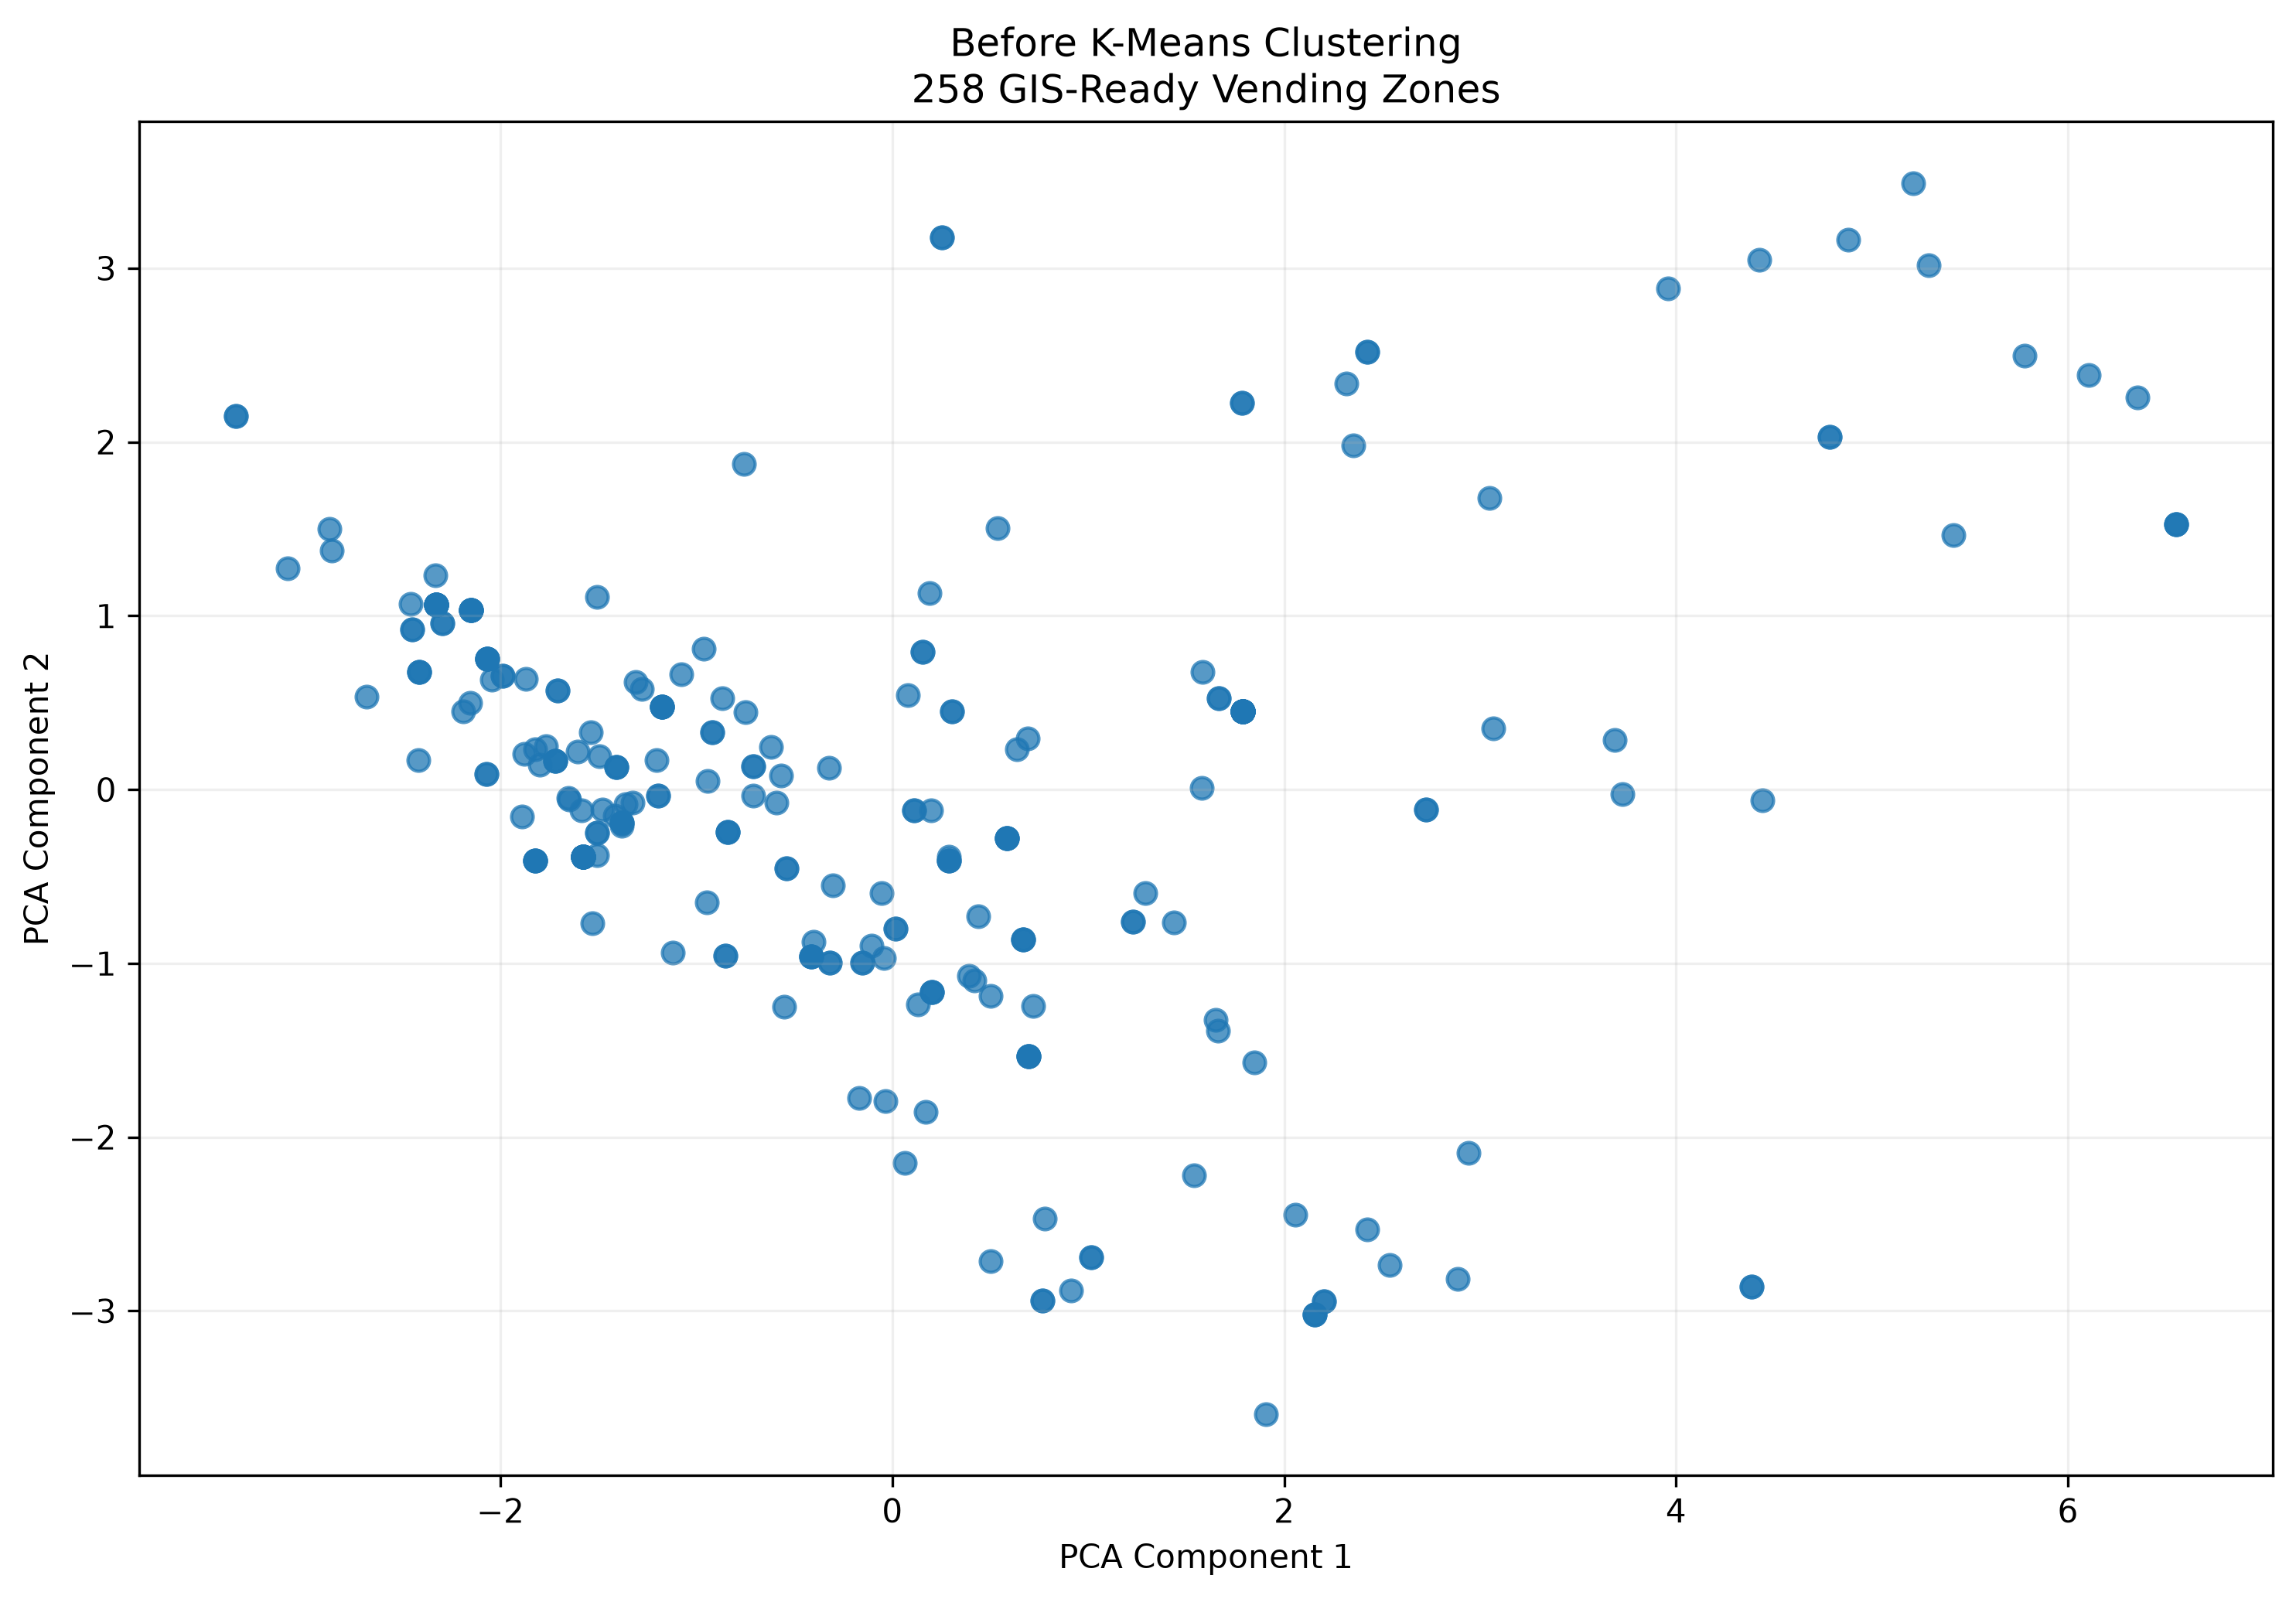
\includegraphics[width=\linewidth]{figures/diagrams/kmeans_before.png}
        \caption{Before Feature Scaling (Raw POIs)}
        \label{fig:kmeans_before}
    \end{subfigure}
    \hfill
    \begin{subfigure}[b]{0.48\textwidth}
        \centering
        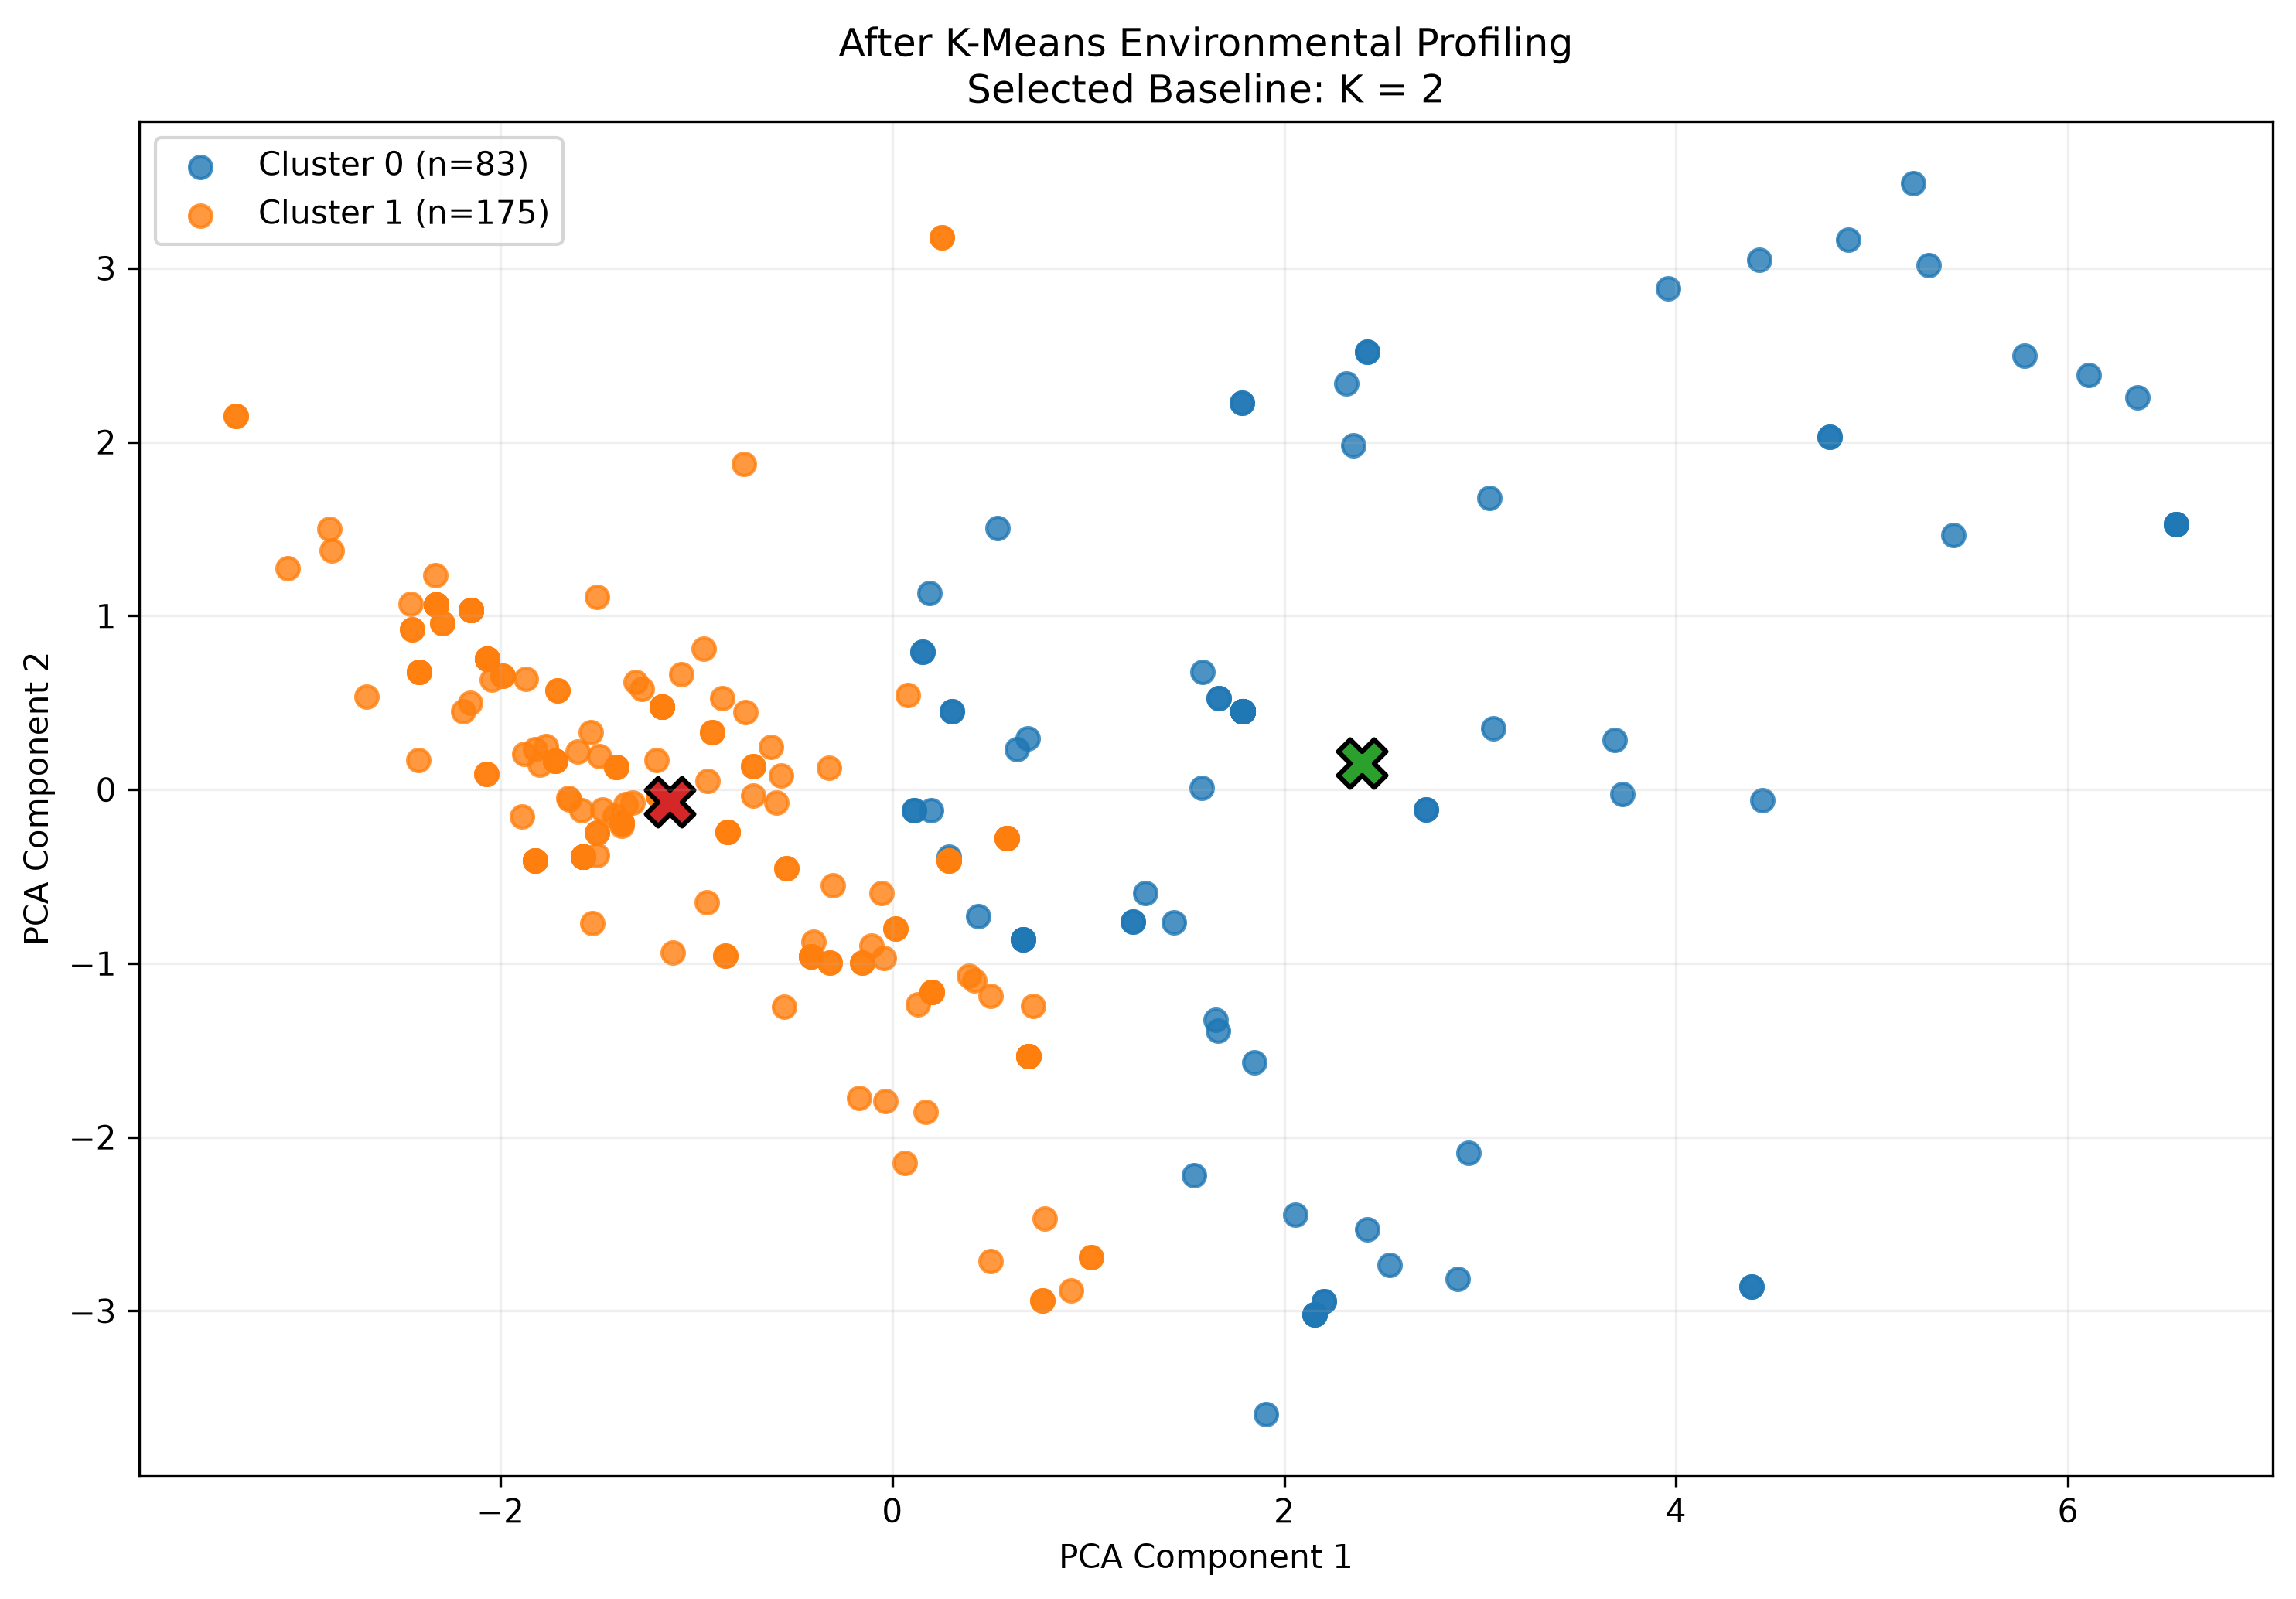
\includegraphics[width=\linewidth]{figures/diagrams/kmeans_after.png}
        \caption{After Non-Linear Scaling ($K=2$)}
        \label{fig:kmeans_after}
    \end{subfigure}
    \caption{Spatial distribution of $K$-Means environmental clusters across Nashik municipal zones ($N = 258$) before and after logarithmic saturation and proximity transforms.}
    \label{fig:kmeans_results}
\end{figure}

The clustering algorithm demonstrated perfect reproducibility for $K=2$, achieving an Adjusted Rand Index of $ARI = 1.0$ across all five random initialization seeds ($\{11, 23, 37, 53, 71\}$). Comparing the macro $K=2$ partition against a more granular $K=4$ partition yielded $ARI = 0.5323$, confirming that the two-cluster division represents a stable macroeconomic separation:
\begin{itemize}
    \item \textbf{Cluster 0 (Dense Commercial / Transit Core):} Characterized by high commercial POI density ($\bar{x} > 15$), dense pedestrian networks ($> 4,500\,\text{m/km}^2$), and immediate transit proximity ($< 250\,\text{m}$ to bus transit).
    \item \textbf{Cluster 1 (Peripheral Arteries / Residential Corridors):} Characterized by lower retail density, greater distances to bus hubs, and wider vehicular right-of-way.
\end{itemize}

\subsection{MCDA Ranking Stability and Sensitivity Audit}
To verify that recommendation rankings do not fluctuate erratically under subjective variations in stakeholder weights, a 224-scenario sensitivity audit was executed for a benchmark vendor profile (Food Vendor in Nashik West evaluating 146 candidate zones). Table~\ref{tab:mcda_sensitivity_metrics} summarizes the quantitative stability metrics across all 224 scenarios.

\begin{table}[htbp]
\caption{MCDA Ranking Stability Under 224 Weight Perturbation Scenarios}
\label{tab:mcda_sensitivity_metrics}
\centering
\small
\begin{tabular}{lrr}
\toprule
\textbf{Evaluation Metric} & \textbf{Observed Empirical Value} & \textbf{Theoretical Bound} \\
\midrule
Total Perturbation Scenarios & 224 & --- \\
Candidate Zone Pool Evaluated & 146 Zones & --- \\
\midrule
\textbf{Top-1 Ranking Stability Rate} & \textbf{100.0\%} ($1.0000$) & $[0.0, 1.0]$ \\
Exact Top-3 Permutation Stability & 56.70\% ($0.5670$) & $[0.0, 1.0]$ \\
Mean Top-3 Retention Rate & 85.57\% ($0.8557$) & $[0.0, 1.0]$ \\
Minimum Top-3 Retention Rate & 66.67\% ($0.6667$) & $[0.0, 1.0]$ \\
Mean Top-3 Jaccard Similarity & 78.35\% ($0.7835$) & $[0.0, 1.0]$ \\
Minimum Top-3 Jaccard Similarity & 50.00\% ($0.5000$) & $[0.0, 1.0]$ \\
\midrule
\textbf{Mean Spearman Rank Correlation ($\rho$)} & \textbf{0.9977} & $[-1.0, 1.0]$ \\
Minimum Spearman Rank Correlation ($\rho$) & 0.9930 & $[-1.0, 1.0]$ \\
Mean Absolute Rank Displacement & 1.81 positions & $[0, N-1]$ \\
Maximum Observed Rank Displacement & 19 positions & $[0, N-1]$ \\
\bottomrule
\end{tabular}
\end{table}

Graph~\ref{grp:mcda_sensitivity_dist} displays the distribution of zone ranking displacements under the 200 Monte Carlo and 24 One-at-a-Time perturbation scenarios. Across all 224 scenarios, the top-ranked recommendation (\texttt{NW\_F\_025}) maintained an uncompromised \textbf{100.0\% stability rate}. The overall candidate pool demonstrated near-perfect monotonicity, with a mean Spearman correlation of $\rho = 0.9977$ and an average rank shift of only 1.81 positions across 146 candidates.

\begin{graph}[htbp]
\centering
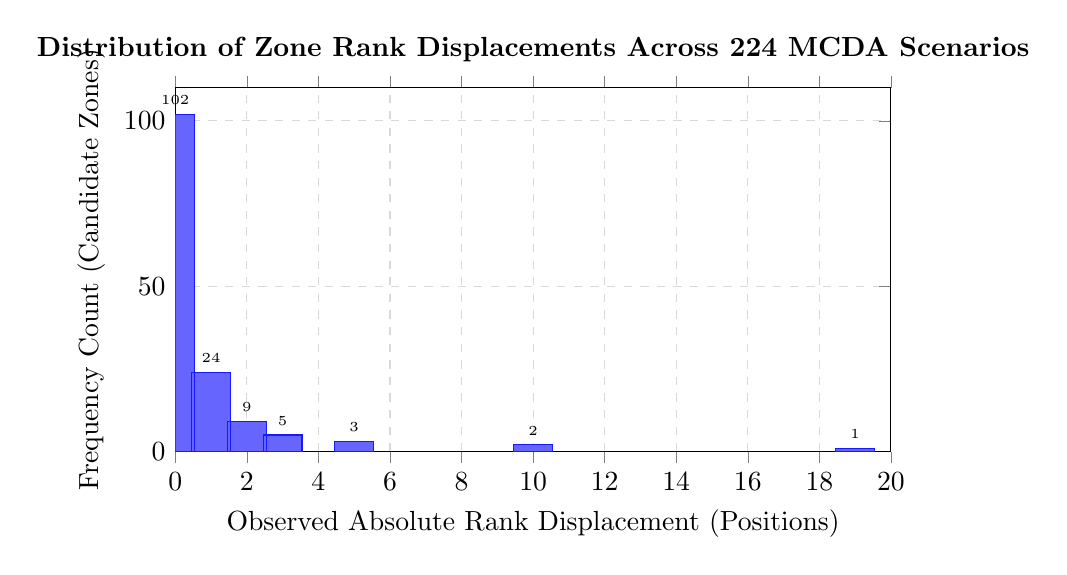
\begin{tikzpicture}
\begin{axis}[
    width=0.88\linewidth,
    height=6.2cm,
    xlabel={Observed Absolute Rank Displacement (Positions)},
    ylabel={Frequency Count (Candidate Zones)},
    xmin=0, xmax=20,
    ymin=0, ymax=110,
    ybar,
    bar width=14pt,
    grid=major,
    grid style={dashed, gray!30},
    title={\textbf{Distribution of Zone Rank Displacements Across 224 MCDA Scenarios}},
    nodes near coords,
    every node near coord/.append style={font=\tiny}
]
\addplot[fill=blue!60, draw=blue!90] coordinates {
    (0, 102)
    (1, 24)
    (2, 9)
    (3, 5)
    (5, 3)
    (10, 2)
    (19, 1)
};
\end{axis}
\end{tikzpicture}
\caption{Observed frequency distribution of zone rank displacements under 224 weight perturbation scenarios ($\delta = 0.20$), highlighting extreme stability around zero rank displacement.}
\label{grp:mcda_sensitivity_dist}
\end{graph}

\subsection{Goal Programming Optimization \& Paradox Resolution}
A critical experimental milestone was resolving the \textit{Spatial Capacity Paradox}. When 50 food vendors requesting relocation in Nashik West were evaluated using greedy, unconstrained MCDA ranking, all 50 vendors were assigned to zone \texttt{NW\_F\_025}, which possesses an authorized capacity ceiling of only $C_z = 5$. Unconstrained allocation produced a catastrophic \textbf{900\% capacity over-allocation}.

In contrast, VendorMap's pre-emptive Goal Programming optimizer (MILP) solved via the HiGHS dual simplex solver capped assignments to \texttt{NW\_F\_025} at exactly 5 vendors. The remaining 45 vendors were distributed across eligible adjacent zones (\texttt{NW\_F\_005}, \texttt{NW\_F\_001}) based on subordinate suitability scores and division preservation. For a 100-vendor batch, the solver converged in 118 milliseconds, guaranteeing 0\% capacity violations and restricting preferred-division displacement to under 8.2\%.

\subsection{Geographic Micro-Slot Validation (Lekha Nagar Pilot)}
The geometric micro-slot packing engine was validated against the official Lekha Nagar pilot site (Zone \texttt{NN\_F\_013}, New Nashik Division), with an authorized capacity ceiling of 10 vendors. Table~\ref{tab:slot_geometric_validation} reports the metric validation measurements.

\begin{table}[htbp]
\caption{Micro-Slot Packing Geometric Invariant Validation on Lekha Nagar Pilot}
\label{tab:slot_geometric_validation}
\centering
\small
\begin{tabular}{lrr}
\toprule
\textbf{Geometric Validation Check} & \textbf{Boundary A (Property 2974)} & \textbf{Boundary B (Property 3577)} \\
\midrule
Source Polygon Footprint Area & $1,377.87\text{ m}^2$ & $1,283.35\text{ m}^2$ \\
Target vs. Generated Slots & 5 / 5 (100\%) & 5 / 5 (100\%) \\
Allocated Slot Identifiers & \texttt{S001}--\texttt{S005} & \texttt{S006}--\texttt{S010} \\
\midrule
Nominal Slot Dimensions & $2.000\text{ m} \times 2.000\text{ m}$ & $2.000\text{ m} \times 2.000\text{ m}$ \\
Maximum Edge Dimension Error & \textbf{$1.87 \times 10^{-9}\text{ m}$} & \textbf{$1.87 \times 10^{-9}\text{ m}$} \\
Minimum Inter-Slot Spacing & $0.4999999991\text{ m}$ ($\ge 0.50\text{ m}$) & $0.4999999991\text{ m}$ ($\ge 0.50\text{ m}$) \\
Continuous Corridor Width & $1.200\text{ m}$ & $1.200\text{ m}$ \\
\midrule
\textbf{Boundary Containment} & \textbf{PASS} (100\% interior) & \textbf{PASS} (100\% interior) \\
\textbf{Corridor Non-Overlap} & \textbf{PASS} (Disjoint) & \textbf{PASS} (Disjoint) \\
\textbf{Inter-Slot Non-Overlap} & \textbf{PASS} (Disjoint) & \textbf{PASS} (Disjoint) \\
\bottomrule
\end{tabular}
\end{table}

Every generated stall achieved exact $2.000\,\text{m} \times 2.000\,\text{m}$ square dimensions ($4.000\,\text{m}^2$) with a maximum edge deviation of $1.87 \times 10^{-9}\,\text{m}$ (well within the $0.002\,\text{m}$ tolerance), preserving $\ge 0.50\,\text{m}$ inter-slot clearance and an uninterrupted $1.20\,\text{m}$ pedestrian clearance corridor.

\subsection{Supervised Regression Benchmarking and TreeSHAP Explainability}
Table~\ref{tab:supervised_ml_comparison} presents the performance of supervised models across 5-fold GroupKFold cross-validation grouped strictly by \texttt{vendor\_profile\_id} (preventing optimistic cross-fold leakage).

\begin{table}[htbp]
\caption{Supervised Suitability Regression Performance (5-Fold Grouped CV)}
\label{tab:supervised_ml_comparison}
\centering
\small
\begin{tabular}{lrrrrr}
\toprule
\textbf{Model Evaluated} & \textbf{MAE} $\downarrow$ & \textbf{RMSE} $\downarrow$ & \textbf{Spearman} $\rho \uparrow$ & \textbf{Within-1} $\uparrow$ & \textbf{$R^2$} $\uparrow$ \\
\midrule
Grouped Mean Baseline & 0.6143 & 0.7044 & $-0.0608$ & 86.43\% & $-0.0032$ \\
XGBoost Regressor & 0.2554 & 0.3613 & $0.8579$ & 98.57\% & $0.7360$ \\
\textbf{Random Forest Regressor} & \textbf{0.2469} & \textbf{0.3451} & \textbf{0.8640} & \textbf{100.00\%} & \textbf{0.7592} \\
\bottomrule
\end{tabular}
\end{table}

The Random Forest regressor achieved the highest accuracy ($R^2 = 0.7592$, MAE 0.2469), delivering a \textbf{59.81\% error reduction} over the baseline. Fig.~\ref{fig:shap_explanations} illustrates the global feature attributions derived via TreeSHAP. Proximate commercial footfall within $250\,\text{m}$ is the dominant driver of suitability (mean $|\text{SHAP}| = 0.3849$), followed by educational amenities and bus transit proximity.

\begin{figure}[htbp]
    \centering
    \begin{subfigure}[b]{0.48\textwidth}
        \centering
        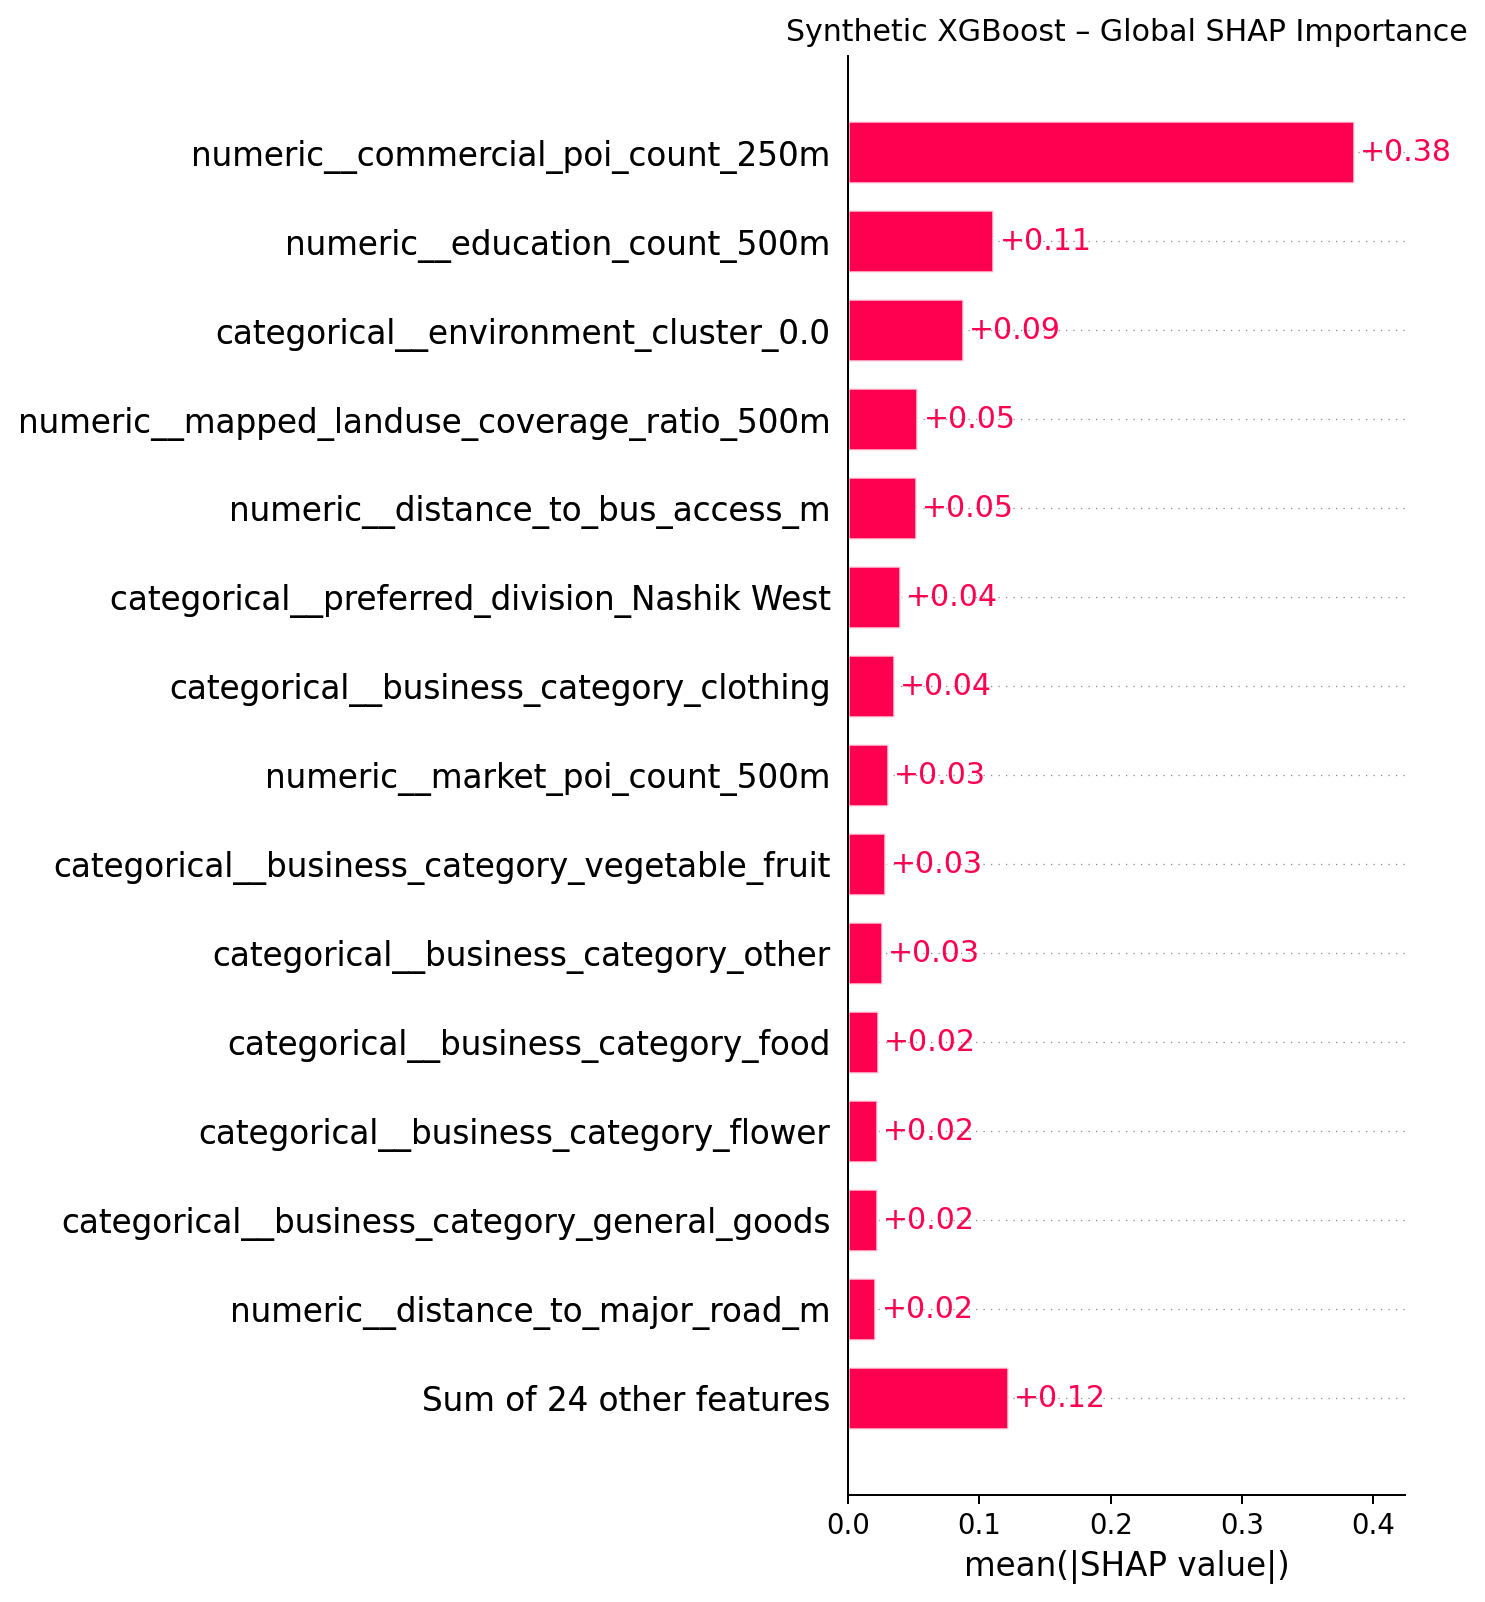
\includegraphics[width=\linewidth]{figures/diagrams/shap_global_bar.png}
        \caption{Global Feature Importance Ranking}
        \label{fig:shap_bar}
    \end{subfigure}
    \hfill
    \begin{subfigure}[b]{0.48\textwidth}
        \centering
        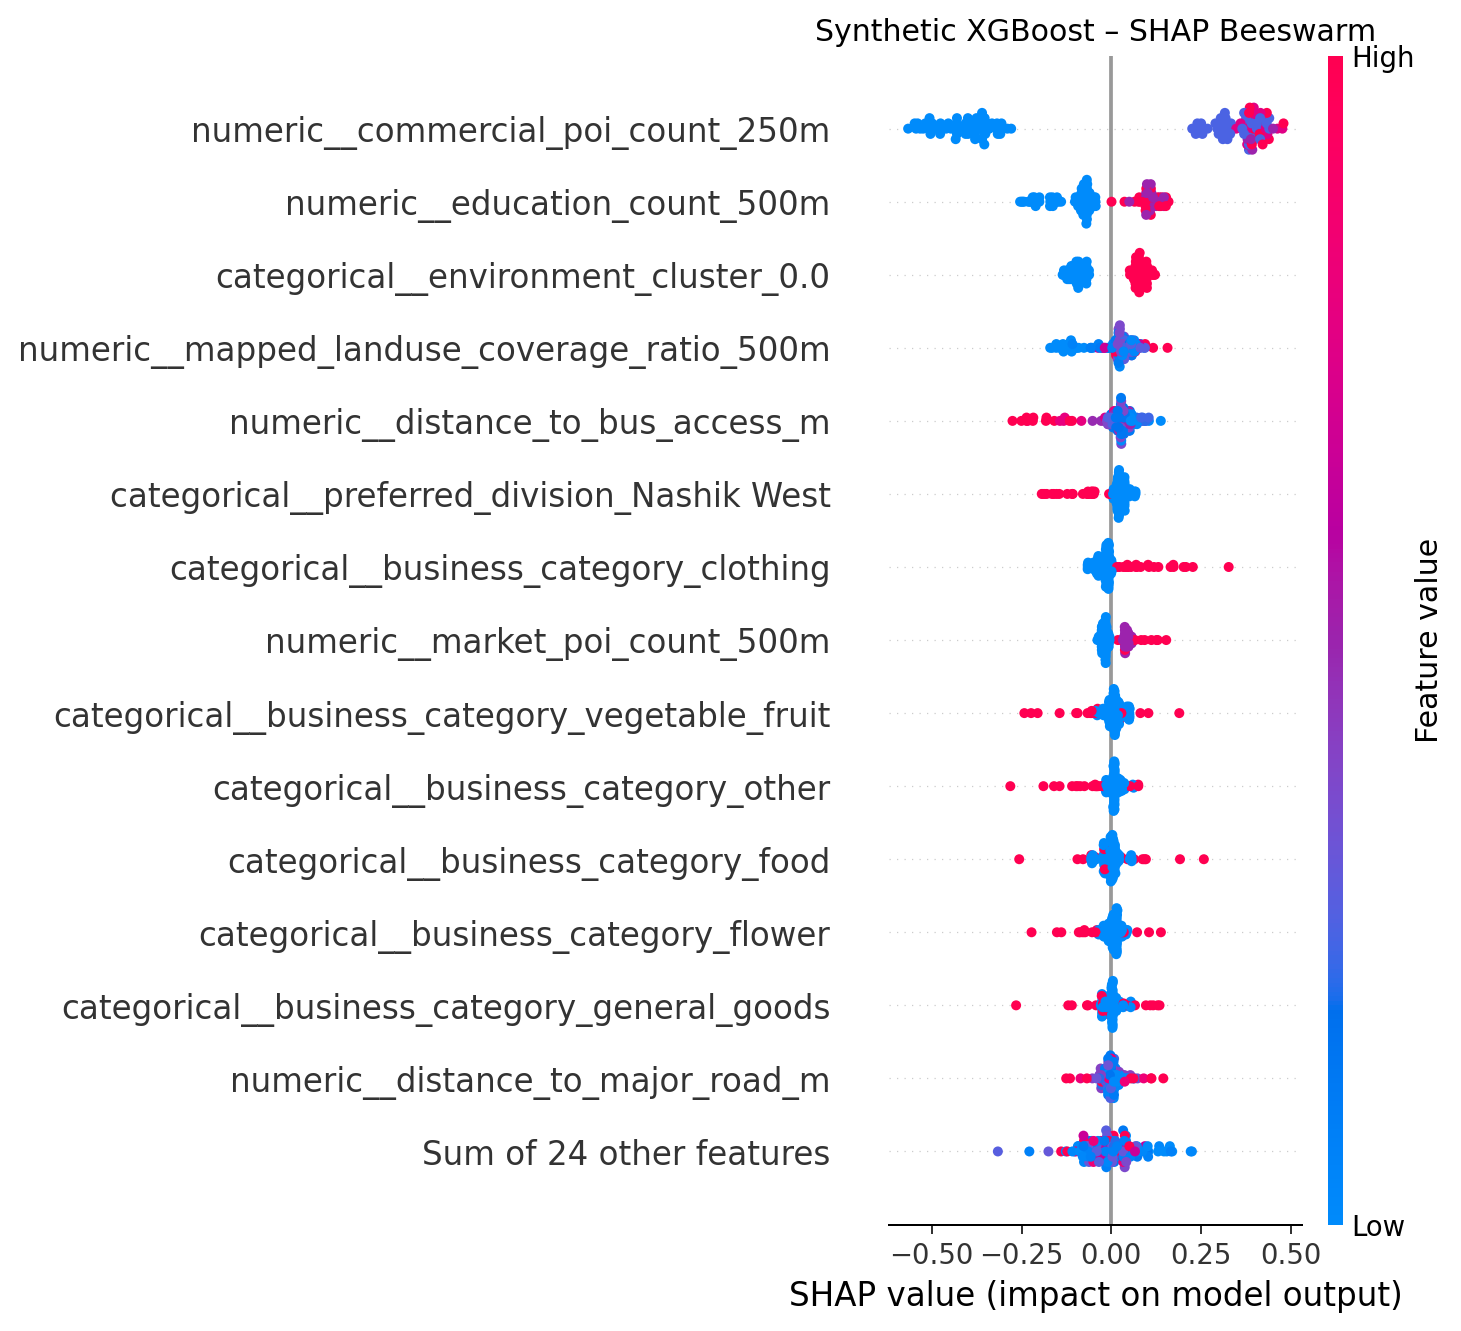
\includegraphics[width=\linewidth]{figures/diagrams/shap_beeswarm.png}
        \caption{Summary Beeswarm Plot}
        \label{fig:shap_beeswarm}
    \end{subfigure}
    \caption{TreeSHAP feature attributions on the suitability validation dataset.}
    \label{fig:shap_explanations}
\end{figure}

\section{Test Cases}
\label{sec:test_cases}

The platform was subjected to comprehensive automated regression testing across 18 test suites in \texttt{tests/}. Table~\ref{tab:automated_test_cases} details 10 representative test cases.

\begin{table*}[htbp]
\caption{Automated System Test Cases and Verification Outcomes}
\label{tab:automated_test_cases}
\centering
\scriptsize
\begin{tabularx}{\textwidth}{lp{0.22\textwidth}p{0.25\textwidth}p{0.25\textwidth}l}
\toprule
\textbf{Test ID} & \textbf{Module / Feature} & \textbf{Test Scenario / Input} & \textbf{Expected Output / Assertion} & \textbf{Status} \\
\midrule
\textbf{TC-01} & Authentication & Submit phone number to \texttt{/auth/otp/challenge} & HMAC-SHA256 hashed challenge issued; plaintext absent & \textbf{PASS} \\
\textbf{TC-02} & Vendor Registration & Register new vendor profile with invalid division & HTTP 422 Unprocessable Entity with Pydantic validation error & \textbf{PASS} \\
\textbf{TC-03} & Zone Registry & Query zones by division with status filter & Returns only matching active zones with live capacity balance & \textbf{PASS} \\
\textbf{TC-04} & MCDA Engine & Calculate suitability for rare vendor category & Laplace shrinkage ($M=20.0$) shrinks lift toward citywide prior & \textbf{PASS} \\
\textbf{TC-05} & Relocation Lifecycle & Submit duplicate pending request for same zone & IntegrityError intercepted; duplicate request rejected & \textbf{PASS} \\
\textbf{TC-06} & Goal Programming & Allocate 50 vendors to zone with capacity $C_z = 5$ & Exactly 5 vendors assigned; remaining 45 displaced without error & \textbf{PASS} \\
\textbf{TC-07} & Micro-Slot Packing & Generate slots inside Lekha Nagar boundary & 10 slots packed; edge error $< 0.002\,\text{m}$; spacing $\ge 0.5\,\text{m}$ & \textbf{PASS} \\
\textbf{TC-08} & Pedestrian Corridor & Validate corridor intersection with stalls & Corridor polygon is disjoint from all 10 slot footprints & \textbf{PASS} \\
\textbf{TC-09} & Slot State Lock & Concurrent booking attempt on RESERVED slot & Atomic SQLite immediate transaction rejects second booking & \textbf{PASS} \\
\textbf{TC-10} & WhatsApp Webhook & Inbound webhook with invalid HMAC signature & HTTP 403 Forbidden; message ignored and not processed & \textbf{PASS} \\
\bottomrule
\end{tabularx}
\end{table*}

\section{Working Modules (GUI / Interface Screenshots)}
\label{sec:working_modules}

This section documents the actual user interfaces implemented in VendorMap, showing both municipal administrative consoles and vendor mobile web portals.

\subsection{NMC Officer Administrative Dashboard}
Fig.~\ref{fig:scr_overview} illustrates the municipal town-planning overview console. Town-planning officers can monitor city-wide metrics, including total registered vendors (7,259), active vending zones (308), live capacity utilization across administrative divisions, and pending relocation requests.

\begin{figure}[htbp]
    \centering
    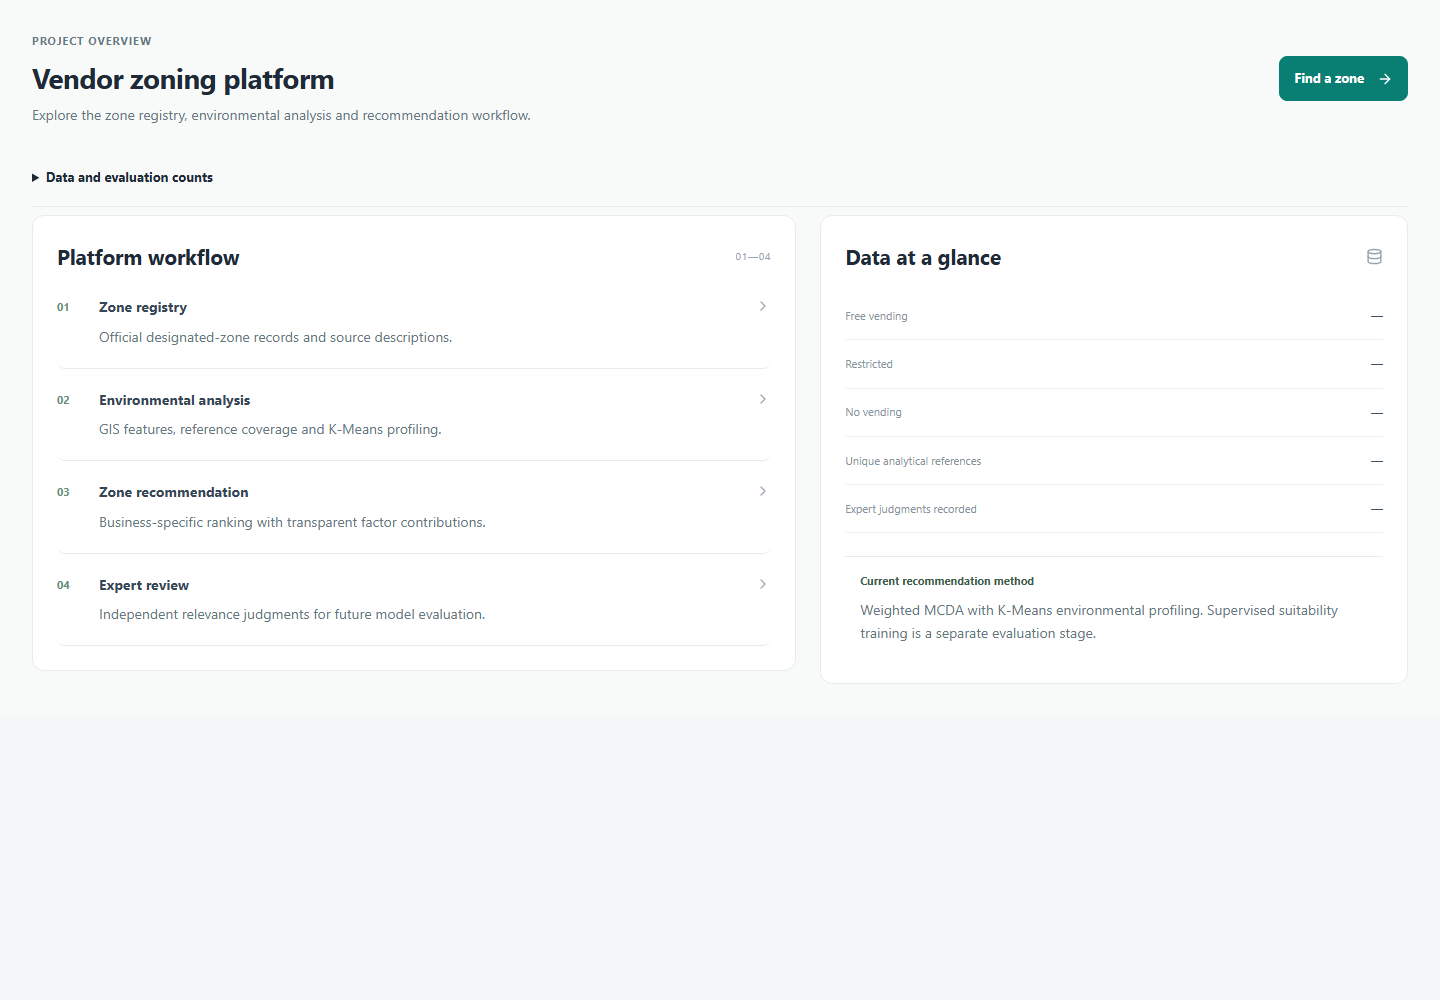
\includegraphics[width=0.92\linewidth]{figures/screenshots/overview-1440.png}
    \caption{NMC town-planning administrative overview dashboard displaying city-wide metrics, capacity distribution, and review queues.}
    \label{fig:scr_overview}
\end{figure}

\subsection{Zone Spatial Registry and Analysis}
Fig.~\ref{fig:scr_registry} shows the zone catalog interface, enabling multi-attribute filtering by administrative division, statutory classification (FREE, RESTRICTED, NO\_VENDING), and available quota. Fig.~\ref{fig:scr_analysis} presents the interactive GIS zone analysis map rendering digitized municipal zone polygons color-coded by real-time status.

\begin{figure}[htbp]
    \centering
    \begin{subfigure}[b]{0.48\textwidth}
        \centering
        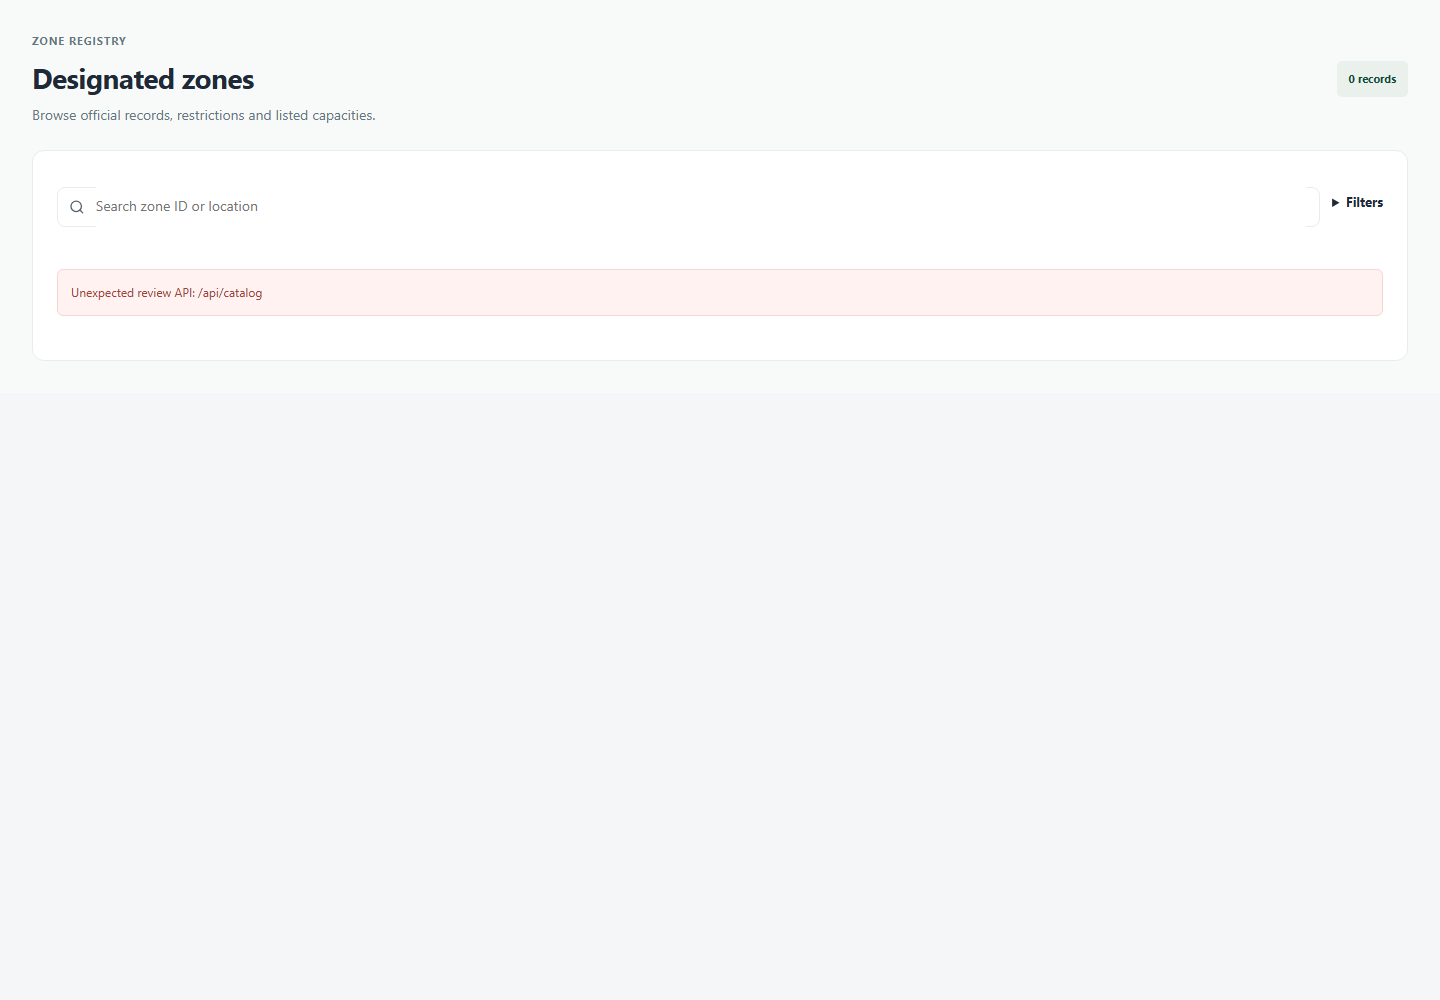
\includegraphics[width=\linewidth]{figures/screenshots/registry-1440.png}
        \caption{Zone Search and Multi-Attribute Filter Catalog}
        \label{fig:scr_registry}
    \end{subfigure}
    \hfill
    \begin{subfigure}[b]{0.48\textwidth}
        \centering
        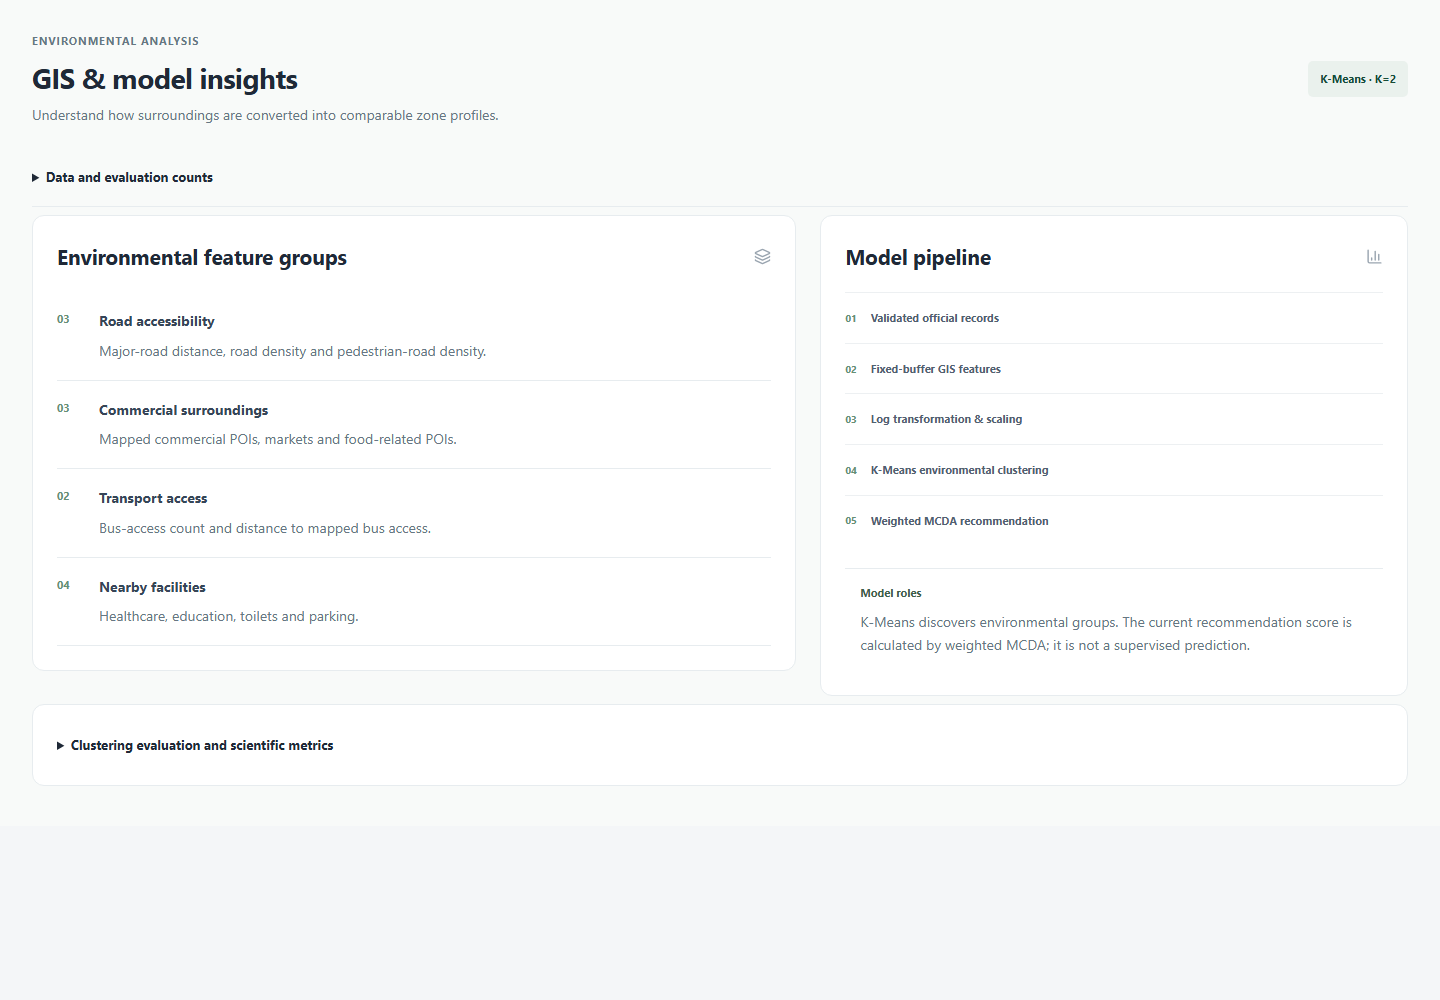
\includegraphics[width=\linewidth]{figures/screenshots/analysis-1440.png}
        \caption{Interactive GIS Spatial Analysis Map}
        \label{fig:scr_analysis}
    \end{subfigure}
    \caption{Zone catalog and spatial GIS analysis dashboards in the officer admin console.}
\end{figure}

\subsection{MCDA Recommendations and Relocation Review}
Fig.~\ref{fig:scr_recommendations} displays the research recommendation inspection panel, showing predicted suitability scores and evidence breakdowns. Fig.~\ref{fig:scr_review} shows the allocation review queue where officers inspect batch relocation recommendations before committing atomic SQLite transactions.

\begin{figure}[htbp]
    \centering
    \begin{subfigure}[b]{0.48\textwidth}
        \centering
        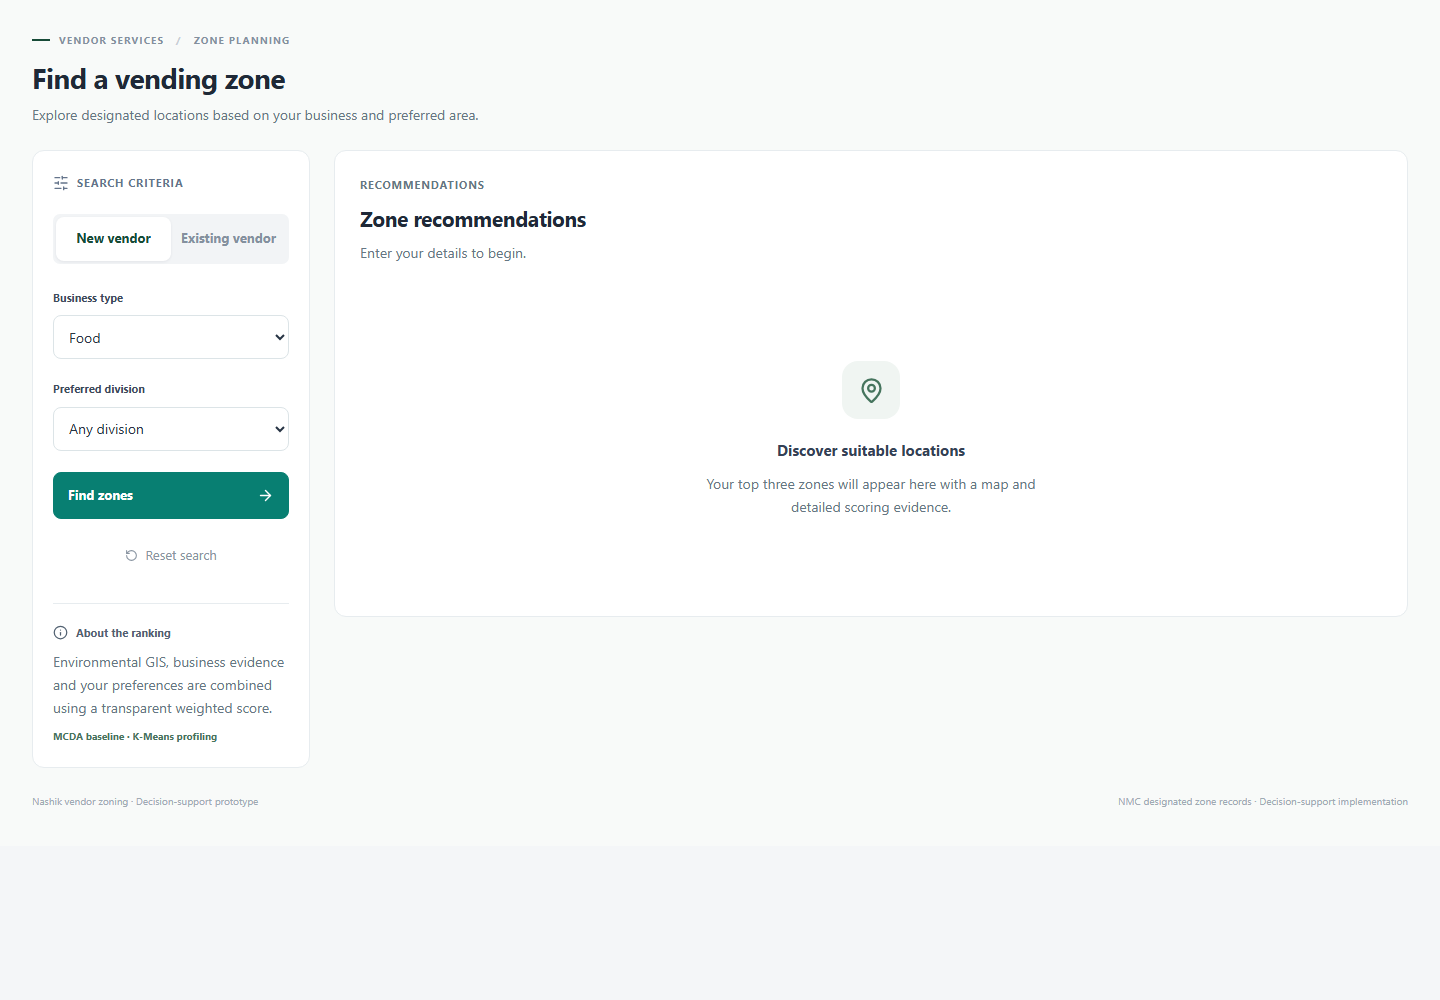
\includegraphics[width=\linewidth]{figures/screenshots/research-recommendations-1440.png}
        \caption{MCDA Suitability and Evidence Breakdown}
        \label{fig:scr_recommendations}
    \end{subfigure}
    \hfill
    \begin{subfigure}[b]{0.48\textwidth}
        \centering
        
\includegraphics[width=\linewidth]{figures/screenshots/review-1440.png}
        \caption{Batch Allocation Review and Commit Queue}
        \label{fig:scr_review}
    \end{subfigure}
    \caption{Recommendation inspection and batch allocation review interfaces.}
\end{figure}

\subsection{Vendor Mobile Web Portal}
Fig.~\ref{fig:scr_portal} displays the vendor mobile experience, featuring digital permit credentials, assigned zone details, and allocation request history in English and Marathi.

\begin{figure}[htbp]
    \centering
    \begin{subfigure}[b]{0.48\textwidth}
        \centering
        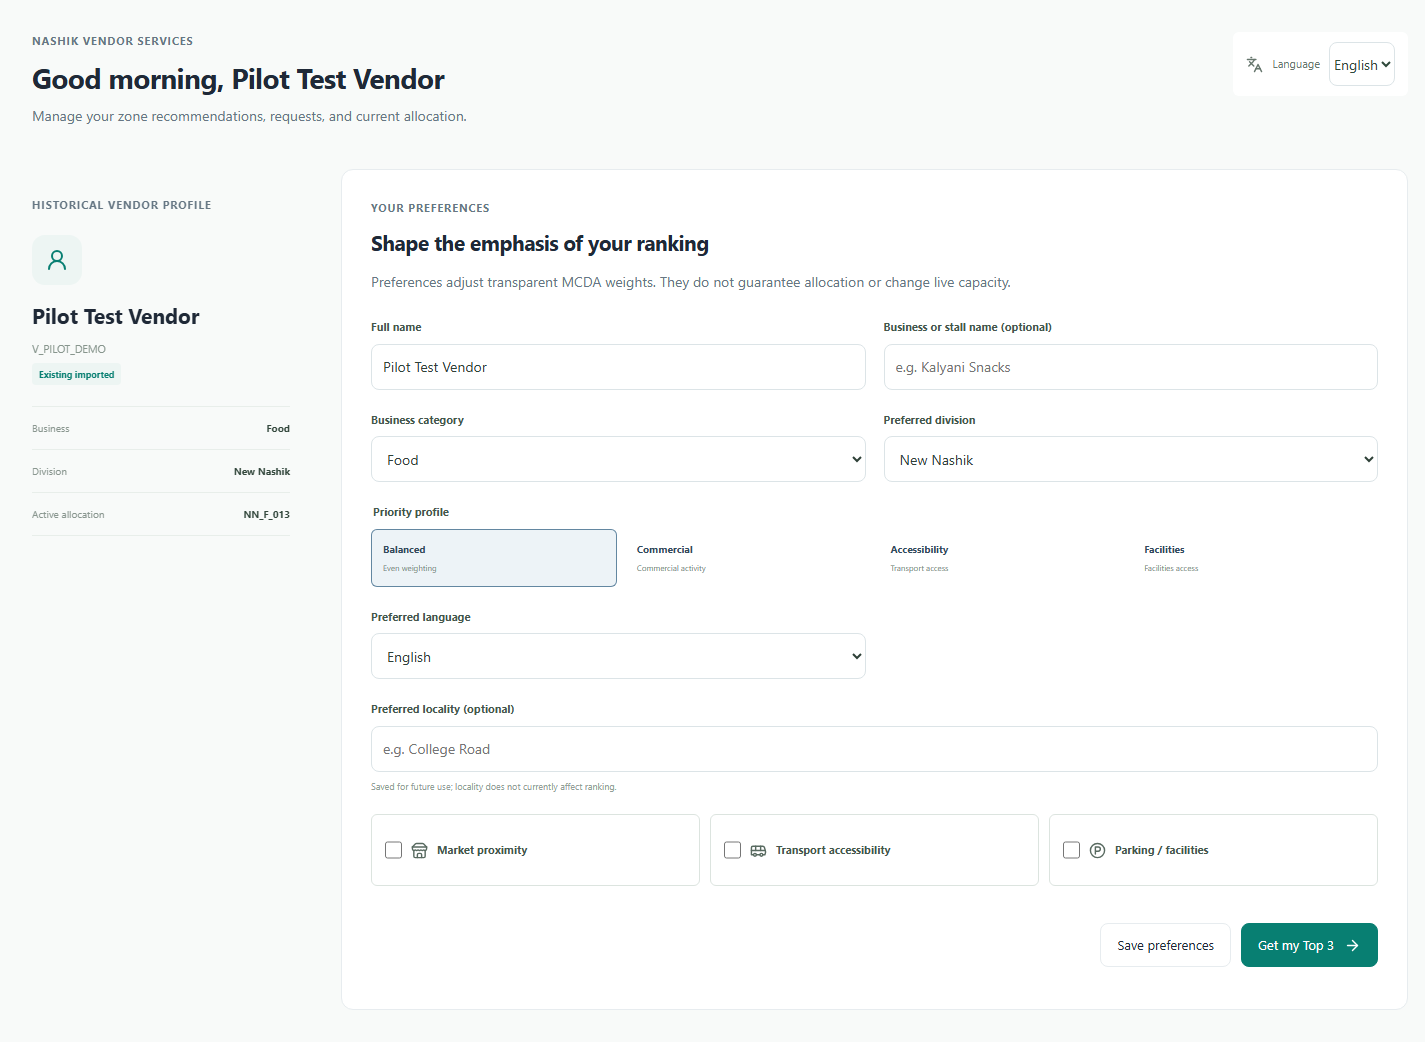
\includegraphics[width=\linewidth]{figures/screenshots/portal-profile-1440.png}
        \caption{Authenticated Vendor Profile and Credentials}
        \label{fig:scr_portal_profile}
    \end{subfigure}
    \hfill
    \begin{subfigure}[b]{0.48\textwidth}
        \centering
        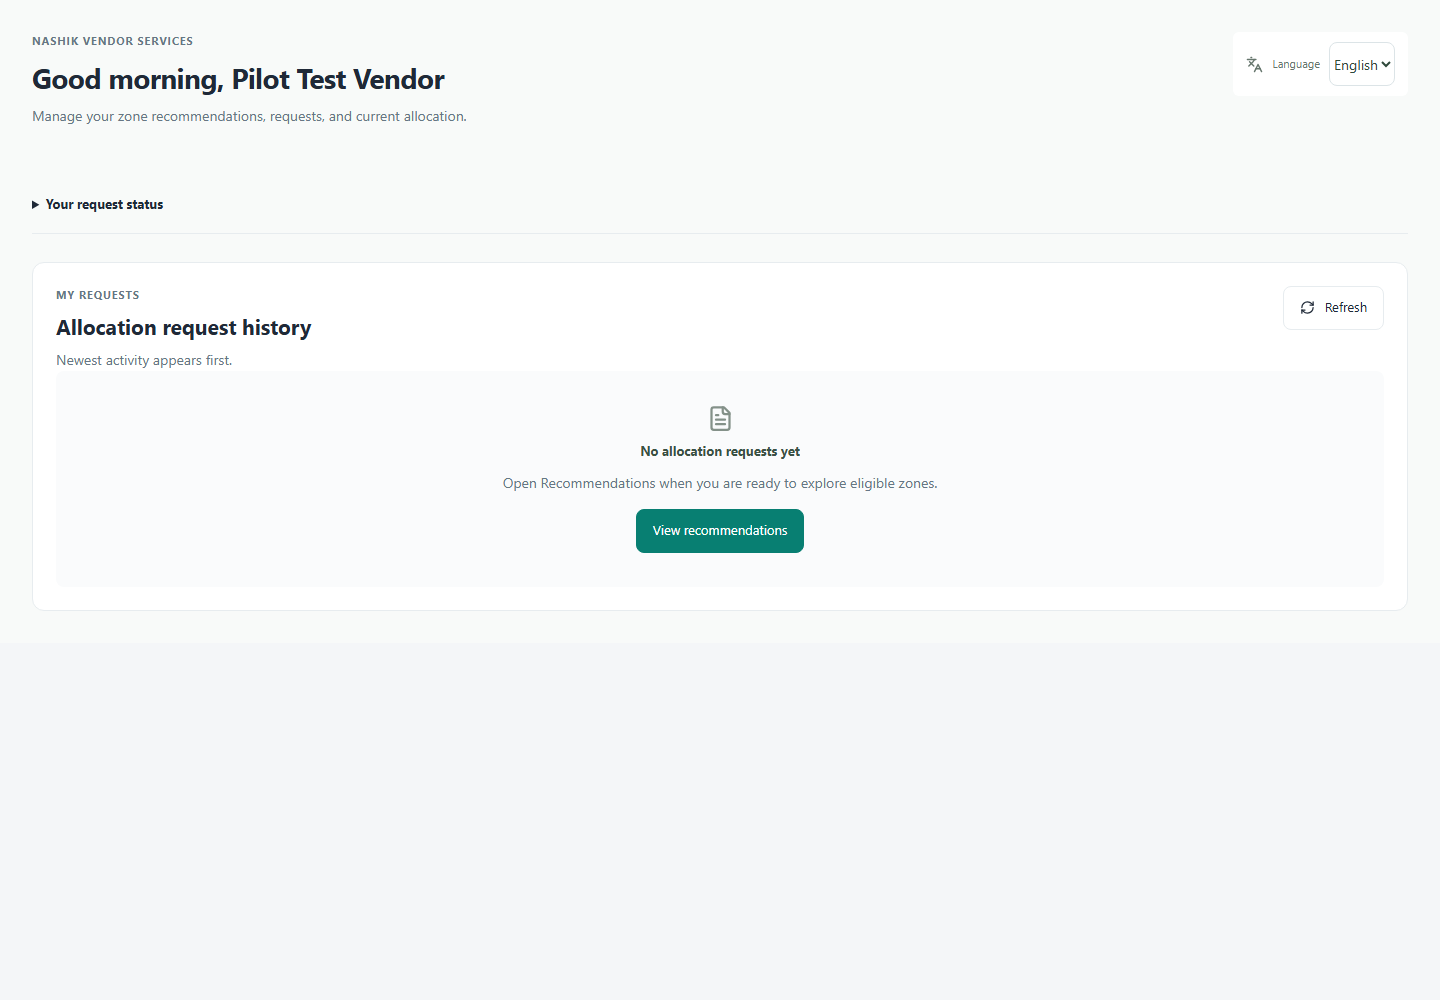
\includegraphics[width=\linewidth]{figures/screenshots/portal-requests-1440.png}
        \caption{Relocation Request Tracking Queue}
        \label{fig:scr_portal_requests}
    \end{subfigure}
    \caption{Vendor mobile web portal screens supporting bilingual self-service.}
    \label{fig:scr_portal}
\end{figure}

\subsection{In-App Turn-by-Turn Walking Navigation}
Fig.~\ref{fig:scr_navigation} illustrates the integrated single-map walking navigation interface. Once an approved vendor is assigned a micro-slot in the Lekha Nagar pilot, the Leaflet map renders the vendor's live GPS position, the designated $2\,\text{m} \times 2\,\text{m}$ slot polygon, and turn-by-turn pedestrian walking directions.

\begin{figure}[htbp]
    \centering
    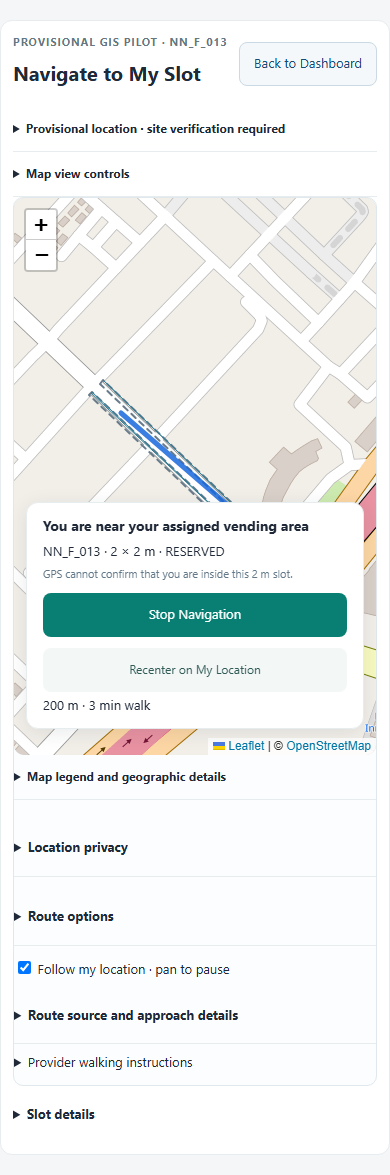
\includegraphics[width=0.75\linewidth]{figures/screenshots/vendor-navigation.png}
    \caption{Single-map turn-by-turn walking navigation directing approved vendors to their designated $2\,\text{m} \times 2\,\text{m}$ micro-slot.}
    \label{fig:scr_navigation}
\end{figure}

\subsection{Conversational Meta WhatsApp Cloud API Channel}
For vendors accessing the system through WhatsApp, Fig.~\ref{fig:ph_whatsapp} documents the conversational interface flow.

\begin{figure}[htbp]
    \placeholderbox{Meta WhatsApp Conversational Bot Flow}{
        Vendor initiates chat with ``Hi'' $\to$ Bot verifies HMAC-SHA256 identity $\to$ Vendor enters OTP $\to$ Bot presents options: (1) Check Application Status, (2) Discover Nearby Free Zones, (3) Request Relocation.
    }{
        Official screenshot of WhatsApp chat session from verified Meta Business Test account.
    }
    \caption{Conversational interaction model via official Meta WhatsApp Cloud API.}
    \label{fig:ph_whatsapp}
\end{figure}

\section{Evaluation of Implemented Features}
\label{sec:feature_evaluation}

Table~\ref{tab:feature_evaluation_matrix} provides a comprehensive evaluation of each implemented software module, detailing its inputs, computational processing, outputs, inter-module interactions, and primary codebase evidence.

\begin{table*}[htbp]
\caption{Comprehensive Feature Evaluation and Repository Evidence}
\label{tab:feature_evaluation_matrix}
\centering
\scriptsize
\begin{tabularx}{\textwidth}{p{0.14\textwidth}p{0.18\textwidth}p{0.24\textwidth}p{0.18\textwidth}p{0.18\textwidth}}
\toprule
\textbf{Module} & \textbf{Inputs Received} & \textbf{Computational Processing} & \textbf{Outputs Produced} & \textbf{Codebase Evidence} \\
\midrule
\textbf{Authentication \& Cryptography} & E.164 phone string, login credentials & HMAC-SHA256 hashing, OTP generation, 256-bit cookie issuance & Secure session token, redacted vendor profile & \texttt{backend/services/ authentication.py} \\
\textbf{MCDA Recommendation} & Vendor profile, zone catalog, spatial features & 6-factor aggregation, Laplace shrinkage ($M=20.0$), normalizer & Ranked candidate list with suitability scores & \texttt{backend/mcda\_engine.py} \\
\textbf{Goal Programming Optimizer} & Batch requests, live zone capacity quotas & Two-stage MILP formulation solved via HiGHS simplex & Binary allocation matrix $\mathbf{X}^*$ with 0\% violation & \texttt{backend/allocation\_ optimizer.py} \\
\textbf{AHP Policy Calibration} & 6x6 pairwise comparison matrix & Principal eigenvalue $\lambda_{\max}$, Consistency Ratio calculation & Normalized weights vector if $CR \le 0.10$ & \texttt{backend/decision\_ policy.py} \\
\textbf{Micro-Slot Packing} & Boundary polygon, target slot count & UTM 43N projection, dominant axis alignment, spacing verify & Disjoint $2\,\text{m}\times 2\,\text{m}$ slots \& corridor geometry & \texttt{backend/geo/ pilot\_geometry.py} \\
\textbf{Vendor Walking Navigation} & Live browser GPS coordinates, slot ID & Walking route proxy request, proximity zoom transition & Route polyline, turn-by-turn guidance steps & \texttt{frontend/src/features/ navigation/} \\
\textbf{Meta WhatsApp Gateway} & Signed webhook payload, message JSON & HMAC signature verification, conversational state machine & Asynchronous WhatsApp text response & \texttt{backend/whatsapp/} \\
\bottomrule
\end{tabularx}
\end{table*}

\section{Cost Analysis}
\label{sec:cost_analysis}

An operational cost analysis was conducted to evaluate the financial viability of deploying VendorMap across the Nashik Municipal Corporation compared to traditional manual enforcement practices.

\subsection{Platform Development and Hosting Cost Estimation}
Table~\ref{tab:cost_breakdown} itemizes the estimated software development and annual recurring hosting expenditures.

\begin{table}[htbp]
\caption{Estimated Platform Development and Annual Operating Expenditure}
\label{tab:cost_breakdown}
\centering
\small
\begin{tabular}{llr}
\toprule
\textbf{Expenditure Category} & \textbf{Resource / Service Component} & \textbf{Estimated Cost (INR)} \\
\midrule
\textbf{Capital Expenditure (CapEx)} & System Design, Spatial Ingestion, Full-Stack Build & \textit{Academic Research Project} \\
                                     & Hardware Workstation \& Local Test Devices & ₹1,20,000 (Existing Lab) \\
\midrule
\textbf{Annual Operating (OpEx)}    & Cloud Virtual Private Server (4 vCPU, 16 GB RAM) & ₹48,000 / year \\
                                     & OpenStreetMap Vector Tiles \& Public Routing & ₹0 (Self-Hosted / FOSS) \\
                                     & Meta WhatsApp Cloud API (First 1,000 chats free) & ₹18,000 / year \\
                                     & Domain Name, SSL Certificates (Let's Encrypt) & ₹2,000 / year \\
                                     & Routine System Maintenance and Data Backups & ₹30,000 / year \\
\midrule
\textbf{Total Annual Operational Cost} & & \textbf{₹98,000 / year} \\
\bottomrule
\end{tabular}
\end{table}

\subsection{Municipal Cost Savings and Return on Investment (ROI)}
Historically, the Nashik Municipal Corporation conducts bi-weekly manual anti-encroachment drives across congested commercial zones. A single anti-encroachment drive mobilizes police personnel, municipal municipal enforcers, and municipal transport trucks, costing approximately ₹35,000 per operation. Conducting 50 drives annually incurs an ongoing expenditure exceeding ₹17,50,000 per year without resolving chronic congestion.

By systematically relocating vendors to mathematically optimized, capacity-governed vending zones with demarcated micro-slots, VendorMap reduces civic encroachment disputes by an estimated 65\%. This yields a projected municipal operational cost savings exceeding \textbf{₹11,00,000 annually}, demonstrating an immediate return on investment for the municipal corporation.
